\subsection{SP0: asignación homogénea uno-a-uno como caso de referencia}
\label{subsec:sp0}

SP0 contiene $N\geq K$ robots homogéneos y $K$ cargas unitarias: cada carga recibe un robot, cada robot atiende como máximo una y la posición solo fija el coste. Este caso bipartito verifica oráculo y métricas antes de introducir heterogeneidad.

Con penalización, los Nash puros coinciden con asignaciones factibles, pero solo los máximos del potencial minimizan coste. Dos Nash pueden tener razón arbitraria (Anexo~\ref{app:proof-sp0-poa}). No hay movimiento, contacto ni red imperfecta.

\subsubsection{Caso base}

La Figura~\ref{fig:sp0-scenario} distingue asociaciones, selección e inactividad. Las aristas representan decisiones y excluyen trayectorias o enlaces.

\begin{figure}[!htbp]
  \centering
  \begin{spdiagram}
    \spdrawarena{SP0 \textbar\ ejemplo bipartito: $N=4$, $K=3$}
    \node[spannotation] at (1.55, 4.37) {$\mathcal R$: robots homogéneos};
    \node[spannotation] at (6.75, 4.37) {$\kappa_{ik}=\bar\delta_{ik}$};
    \node[spannotation] at (11.90, 4.37) {$\mathcal L$: cargas unitarias};

    \node[sprobot] (r1) at (1.45, 3.60) {$R_1$};
    \node[sprobot] (r2) at (1.45, 2.65) {$R_2$};
    \node[sprobot] (r3) at (1.45, 1.85) {$R_3$};
    \node[sprobotfree,scale=0.82] (r4) at (1.45, 1.08) {$R_4$};
    \node[spmuted,anchor=west] at (1.78, 1.08) {$a_4=0$};

    \node[spload] (l1) at (12.00, 3.60) {$L_1$};
    \node[spload] (l2) at (12.00, 2.65) {$L_2$};
    \node[spload] (l3) at (12.00, 1.85) {$L_3$};

    \draw[spcandidate,-,opacity=0.72] (r1) -- (l2);
    \draw[spcandidate,-,opacity=0.72] (r2) -- (l1);
    \draw[spcandidate,-,opacity=0.72] (r2) -- (l3);
    \draw[spcandidate,-,opacity=0.72] (r3) -- (l2);
    \draw[spcandidate,-,opacity=0.72] (r4) -- (l3);
    \draw[spassign,solid,-,line width=1.25pt] (r1) -- node[spannotation,pos=0.53] {$x_{11}=1$} (l1);
    \draw[spassign,solid,-,line width=1.25pt] (r2) -- node[spannotation,pos=0.53] {$x_{22}=1$} (l2);
    \draw[spassign,solid,-,line width=1.25pt] (r3) -- node[spannotation,pos=0.53] {$x_{33}=1$} (l3);

    \draw[spassign,solid,-,line width=1.25pt] (0.75, 0.34) -- (1.45, 0.34);
    \node[splegend,anchor=west] at (1.58, 0.34) {seleccionada: $x_{ik}=1$};
    \draw[spcandidate,-] (4.70, 0.34) -- (5.40, 0.34);
    \node[splegend,anchor=west] at (5.53, 0.34) {alternativa: $x_{ik}=0$};
    \node[sprobotfree,scale=0.45] at (9.65, 0.34) {};
    \node[splegend,anchor=west] at (9.90, 0.34) {robot libre: $a_i=0$};
  \end{spdiagram}
  \caption{SP0: asociaciones admisibles (gris), selección final (azul) y robot libre para $N>K$. La figura no representa movimiento ni comunicación.}
  \label{fig:sp0-scenario}
  \viuownsource
\end{figure}

Sean $p_i,p_k^L\in\mathbb R^2$ las posiciones del robot $i$ y de la carga $k$. Con una cota geométrica $\delta_{\max}>0$ fijada antes de resolver, el coste adimensional es
\begin{equation}
 \delta_{ik}=\lVert p_i-p_k^L\rVert_2\ [\mathrm m],\qquad
 \bar\delta_{ik}=\frac{\delta_{ik}}{\delta_{\max}},\qquad
 \kappa_{ik}=\bar\delta_{ik}\in[0, 1].
    \label{eq:sp0-distance-cost}
\end{equation}
La salida es una asociación lógica, sin trayectoria ni control. SP3 introduce contacto y SP4 transporte.

\subsubsection{Formulación exacta y oráculo de asignación}

Con $\Robots=\{1,\ldots,N\}$, $\Loads=\{1,\ldots,K\}$ y $x_{ik}\in\{0, 1\}$, el oráculo central resuelve
\begin{equation}
\label{eq:sp0-oracle}
\begin{aligned}
 C^\star=\min_x\quad &\sum_{i\in\Robots}\sum_{k\in\Loads}\kappa_{ik}x_{ik}\\
 \text{sujeto a}\quad &\sum_{k\in\Loads}x_{ik}\leq1 &&(i\in\Robots),\\
 &\sum_{i\in\Robots}x_{ik}=1 &&(k\in\Loads).
\end{aligned}
\end{equation}
Es el problema lineal de asignación: su relajación tiene vértices enteros y el húngaro lo resuelve en $O(N^3)$ tiempo y $O(N^2)$ memoria \parencite{kuhn1955Hungarian}. SP0 pertenece a $\mathsf P$. La integralidad y la extensión con mochila 0--1 se prueban en el Anexo~\ref{app:proof-sp0-complexity}.

El oráculo recibe la matriz completa y no representa la arquitectura propuesta. Para un perfil $a$, el experimento usa
\begin{equation}
 \begin{aligned}
 C(a)&=\sum_{i:a_i\neq0}\kappa_{i,a_i}, &
 r(a)&=\frac{C(a)-C^\star}{K},\\
 W_\lambda(a)&=BK-F_\lambda(a), &
 \eta_W(a)&=\frac{W_\lambda(a)}{BK-C^\star},\qquad B=1.05.
 \end{aligned}
 \label{eq:sp0-evaluation-metrics}
\end{equation}
La brecha $r$ solo se informa si hay factibilidad. $\eta_W$ se muestra como $100W/W^\star$. Las \emph{operaciones registradas} no son comparables entre algoritmos: cuentan entradas/aristas, utilidades por puja, acciones o pares candidatos según el método.

Como $0\leq\kappa_{ik}\leq1$, $B=1.05$ garantiza $BK-C^\star\geq0.05K$ y evita dividir por cero. Solo escala el bienestar. No altera orden, oráculo ni pagos.

\subsubsection{Juego potencial y caracterización de los equilibrios}

\begin{contribucion}{formulación y caracterización del juego de SP0}
Cada robot elige $a_i\in\{0\}\cup\Loads$, donde $0$ denota inactividad. Con $m_k(a)=\sum_i\mathbf1\{a_i=k\}$, se definen el déficit, el exceso y el coste penalizado
\begin{equation}
\begin{aligned}
 D(a)&=\sum_k\positivepart{1-m_k(a)}, &
 E(a)&=\sum_k\positivepart{m_k(a)-1},\\
 C(a)&=\sum_{i:a_i\neq0}\kappa_{i,a_i}, &
 F_\lambda(a)&=C(a)+\lambda\{D(a)+E(a)\}.
\end{aligned}
\label{eq:sp0-penalized-cost}
\end{equation}
La función potencial es $\Phi_\lambda=-F_\lambda$ y el pago marginal es $u_i(a)=\Phi_\lambda(a)-\Phi_\lambda(0,a_{-i})$. La fitness de escoger $k$ es
\begin{equation}
 f_{ik}(a_{-i})=
 \begin{cases}
  \lambda-\kappa_{ik},&m_k(a_{-i})=0,\\
  -\lambda-\kappa_{ik},&m_k(a_{-i})\geq1,
 \end{cases}
 \qquad f_{i0}=0.
 \label{eq:sp0-action-fitness}
\end{equation}
Todos los términos son adimensionales. La activación revisa un robot por evento y adopta una mejora estricta. Prescinde de rondas globales de decisión y presupone una ocupación lógica coherente.

\begin{proposicion}[Factibilidad y selección en SP0]
\label{thm:sp0-nash-characterization}
Si $N\geq K$ y $\lambda>\kappa_{\max}$, entonces se cumplen cinco propiedades. \emph{(i)} El juego es de potencial exacto. \emph{(ii)} Sus Nash puros son exactamente las asignaciones factibles. \emph{(iii)} Toda secuencia de mejoras estrictas es finita y termina en un Nash. \emph{(iv)} Los máximos globales del potencial coinciden con las soluciones de \eqref{eq:sp0-oracle}. \emph{(v)} Un Nash cualquiera puede ser subóptimo.
\end{proposicion}
\end{contribucion}
Cubrir un vacío o retirar un duplicado mejora el pago porque $\lambda$ supera el coste. Ningún perfil con déficit o exceso es Nash. Desde una asignación factible, toda desviación crea uno de ambos. Solo las de coste mínimo maximizan el potencial (Anexo~\ref{app:sp0-proofs}).

\begin{corolario}[Precios de estabilidad y anarquía de SP0]
\label{cor:sp0-pos-poa}
Con coste social $C$ restringido a asignaciones factibles y bajo los supuestos de
la Proposición~\ref{thm:sp0-nash-characterization}, el precio de estabilidad es
$\operatorname{PoS}_0=1$. El precio de la anarquía no admite una cota uniforme:
$\operatorname{PoA}_0=+\infty$ sobre la familia de instancias normalizadas con
coste óptimo positivo.
\end{corolario}
El óptimo social pertenece al conjunto de Nash. En cambio, la familia
$\boldsymbol\kappa_\epsilon$ del Anexo~\ref{app:proof-sp0-poa} contiene un Nash
de coste $1$ y un óptimo de coste $2\epsilon$, por lo que la razón diverge al
hacer $\epsilon\downarrow0$. La existencia de un equilibrio óptimo no controla
la eficiencia del equilibrio seleccionado por una trayectoria local.

La penalización garantiza cobertura y exclusividad. La selección eficiente requiere un criterio adicional. El 2-intercambio amplía el vecindario de mejora y puede corregir equilibrios unilaterales, aunque solo certifica estabilidad frente a los pares examinados.

\subsubsection{Métodos comparados}

Se comparan húngaro, subasta-$\varepsilon$, voraz y dos mejores respuestas. Los dos primeros globales conocen la matriz. Mejor respuesta usa costes propios y ocupación agregada. $\lambda=0$ es ablación. En la Tabla~\ref{tab:sp0-method-literature}, $m=\max\{N,K\}$, $B_\varepsilon$ cuenta pujas e $I_{\mathrm{BR}},I_2$ barridos.

\begin{table}[!htbp]
 \centering
 \caption{Comparación computacional de métodos en SP0.}
 \label{tab:sp0-method-literature}
 \scriptsize
 \setlength{\tabcolsep}{1.5pt}
 \renewcommand{\arraystretch}{1.04}
 \begin{tabularx}{\textwidth}{>{\raggedright\arraybackslash}p{2.25cm} >{\raggedright\arraybackslash}p{1.45cm} >{\raggedright\arraybackslash}p{2.25cm} >{\raggedright\arraybackslash}p{2.15cm} >{\raggedright\arraybackslash}p{1.55cm} Y}
  \toprule
  Método/fuente & Clase & Coste & Arq./información & Parámetros & Garantía/límite \\
  \midrule
  Algoritmo húngaro \parencite{kuhn1955Hungarian} & LAP en P & $O(m^3)$ tiempo; $O(NK)$ memoria & Central; matriz $\boldsymbol\kappa$ completa & Desempate & Óptimo global del LAP. \\
  Subasta-$\varepsilon$ \parencite{bertsekas1988Auction} & LAP en P & $O(KB_\varepsilon)$; $B_\varepsilon$ depende del rango y $\varepsilon$ & Precios/ganadores compartidos; sin red vecinal & $\varepsilon$ & Brecha aditiva $\leq N\varepsilon$. No demuestra ejecución distribuida. \\
  Método voraz (familia de mercado \parencite{gerkeyMataric2002MURDOCH}) & LAP en P; heurística & $O(NK\log(NK))$ & Central; lista global de aristas & Orden/desempate & Factible. No equivale a MURDOCH y carece de cota. \\
  Mejor respuesta \parencite{monderer1996potential} & Equilibrio de juego finito & $O(I_{\mathrm{BR}}NK)$; a lo sumo $(K+1)^N-1$ mejoras estrictas & Local con ocupación agregada exacta & $\lambda$, orden, $I_{\max}$ & Termina en Nash factible si $\lambda>\kappa_{\max}$. No es óptimo social. \\
  Mejor respuesta + 2-intercambio & Búsqueda local & $O(I_2N^2)$ pares, con costes cacheados & Bilateral sobre asignación vigente & $I_{2,\max}$, desempate & Estable solo frente a los intercambios examinados. \\
  \bottomrule
 \end{tabularx}
 \viuownsource
\end{table}

\subsubsection{Dinámica de revisión}

SP0 no integra planta, pero regula el perfil discreto $a$ mediante la salida
\begin{equation}
 \boldsymbol z_0(a)=
 \begin{bmatrix}D(a)&E(a)\end{bmatrix}^{\mathsf T},
 \qquad
 \boldsymbol z_0^{\mathrm{ref}}=\boldsymbol 0.
 \label{eq:sp0-strategic-regulation}
\end{equation}
Sus componentes cuentan vacíos y duplicados. $\nu_i$ revisa una acción y carece de unidades de velocidad. Usa $\kappa_{i\cdot}$ y $\widehat m_{ik}=m_k(a)$, ocupación global exacta.

Con activación asíncrona, la ley de realimentación ejecutada es
\begin{equation}
 a_i^+\in\argmax_{b\in\mathcal A_i}u_i(b,a_{-i}),
 \qquad
 \nu_i=
 \begin{cases}
  a_i^+,&u_i(a_i^+,a_{-i})>u_i(a),\\
  a_i,&\text{en otro caso}.
 \end{cases}
 \label{eq:sp0-feedback-law}
\end{equation}
El oráculo selecciona coste mínimo. El lazo solo regula cobertura y exclusividad. $\boldsymbol z_0=0$ no implica optimalidad.

\begin{corolario}[Regulación estratégica finita de SP0]
\label{cor:sp0-strategic-regulation}
Si $N\geq K$, $\lambda>\kappa_{\max}$, la ocupación realimentada es coherente y la activación no deja indefinidamente sin revisar a un robot con mejora estricta, la ley~\eqref{eq:sp0-feedback-law} alcanza en un número finito de revisiones el conjunto $\{a:\boldsymbol z_0(a)=\boldsymbol0\}$.
\end{corolario}
Cada actualización reduce $F_\lambda$ en un espacio finito y todo Nash cumple $D=E=0$ (Anexo~\ref{app:sp0-proofs}). Es una estabilización lógica por eventos. Quedan fuera la estabilidad física y la dinámica continua.

\paragraph{Certificado con copias locales de precios.}
El experimento usa ocupación global. Como resultado complementario, el Anexo~\ref{app:proof-sp0-local-prices} audita una asignación factible $\sigma_t$ mediante precios locales. Si cada robot satisface complementariedad $\varepsilon$ y las copias difieren del precio promedio a lo sumo en $e_\pi^t$, entonces
\begin{equation}
 0\leq C(\sigma_t)-C^\star\leq N(\varepsilon+2e_\pi^t).
 \label{eq:sp0-local-price-gap}
\end{equation}
Con consenso lineal sobre un grafo conexo, $e_\pi^t\leq q^t\mathcal D_0$, donde $\mathcal D_0:=\lVert[\widehat{\boldsymbol\pi}_i^0-\bar{\boldsymbol\pi}^0]_{i=1}^N\rVert_F$ es el desacuerdo inicial apilado y $q<1$ depende del espectro de $I-\alpha L$. De ahí se obtiene un coste suficiente de $2|\mathcal E_C|Nt_\eta$ escalares para alcanzar tolerancia $\eta$. Con costes enteros, una cota menor que uno certifica optimalidad. Una partición permanente impide una garantía uniforme porque existen matrices globales distintas e indistinguibles desde una componente.
\subsubsection{Diseño experimental}

Se generaron 200 instancias pareadas mediante posiciones uniformes en el cuadrado unidad: $N\in\{4, 8, 16, 32, 64\}$, $K/N\in\{0.5, 1\}$ y 20 semillas por combinación. Los métodos recibieron las mismas matrices de coste. Se fijaron $\lambda=\kappa_{\max}+0.05$ y $\varepsilon=10^{-3}$. Además, 21 instancias pequeñas se enumeraron exhaustivamente. Se registraron factibilidad, déficit, exceso, coste, brecha por carga, bienestar relativo, operaciones y CPU. Los intervalos se calcularon mediante 2000 remuestras pareadas de instancias independientes. Los contratos de información no son equivalentes y no se evaluó una red.

\subsubsection{Resultados}

\paragraph{Caracterización formal.}
Las 21 enumeraciones confirmaron la Proposición~\ref{thm:sp0-nash-characterization}. Para $N=K=5$ hubo $120$ Nash entre $7776$ perfiles y una única asignación óptima ($0.833\%$ de los equilibrios): factibilidad no selecciona eficiencia.

El conjunto de equilibrios crece factorialmente y su brecha frente al oráculo presenta una dispersión amplia. Los cinco métodos completos alcanzaron la misma factibilidad, por lo que esa medida se informa en el texto y la tabla conserva las cifras de selección.

% Gráfico generado conservado como artefacto suplementario; la tabla contiene
% los valores exactos usados en la inferencia.
\iffalse
\begin{figure}[!htbp]
 \centering
 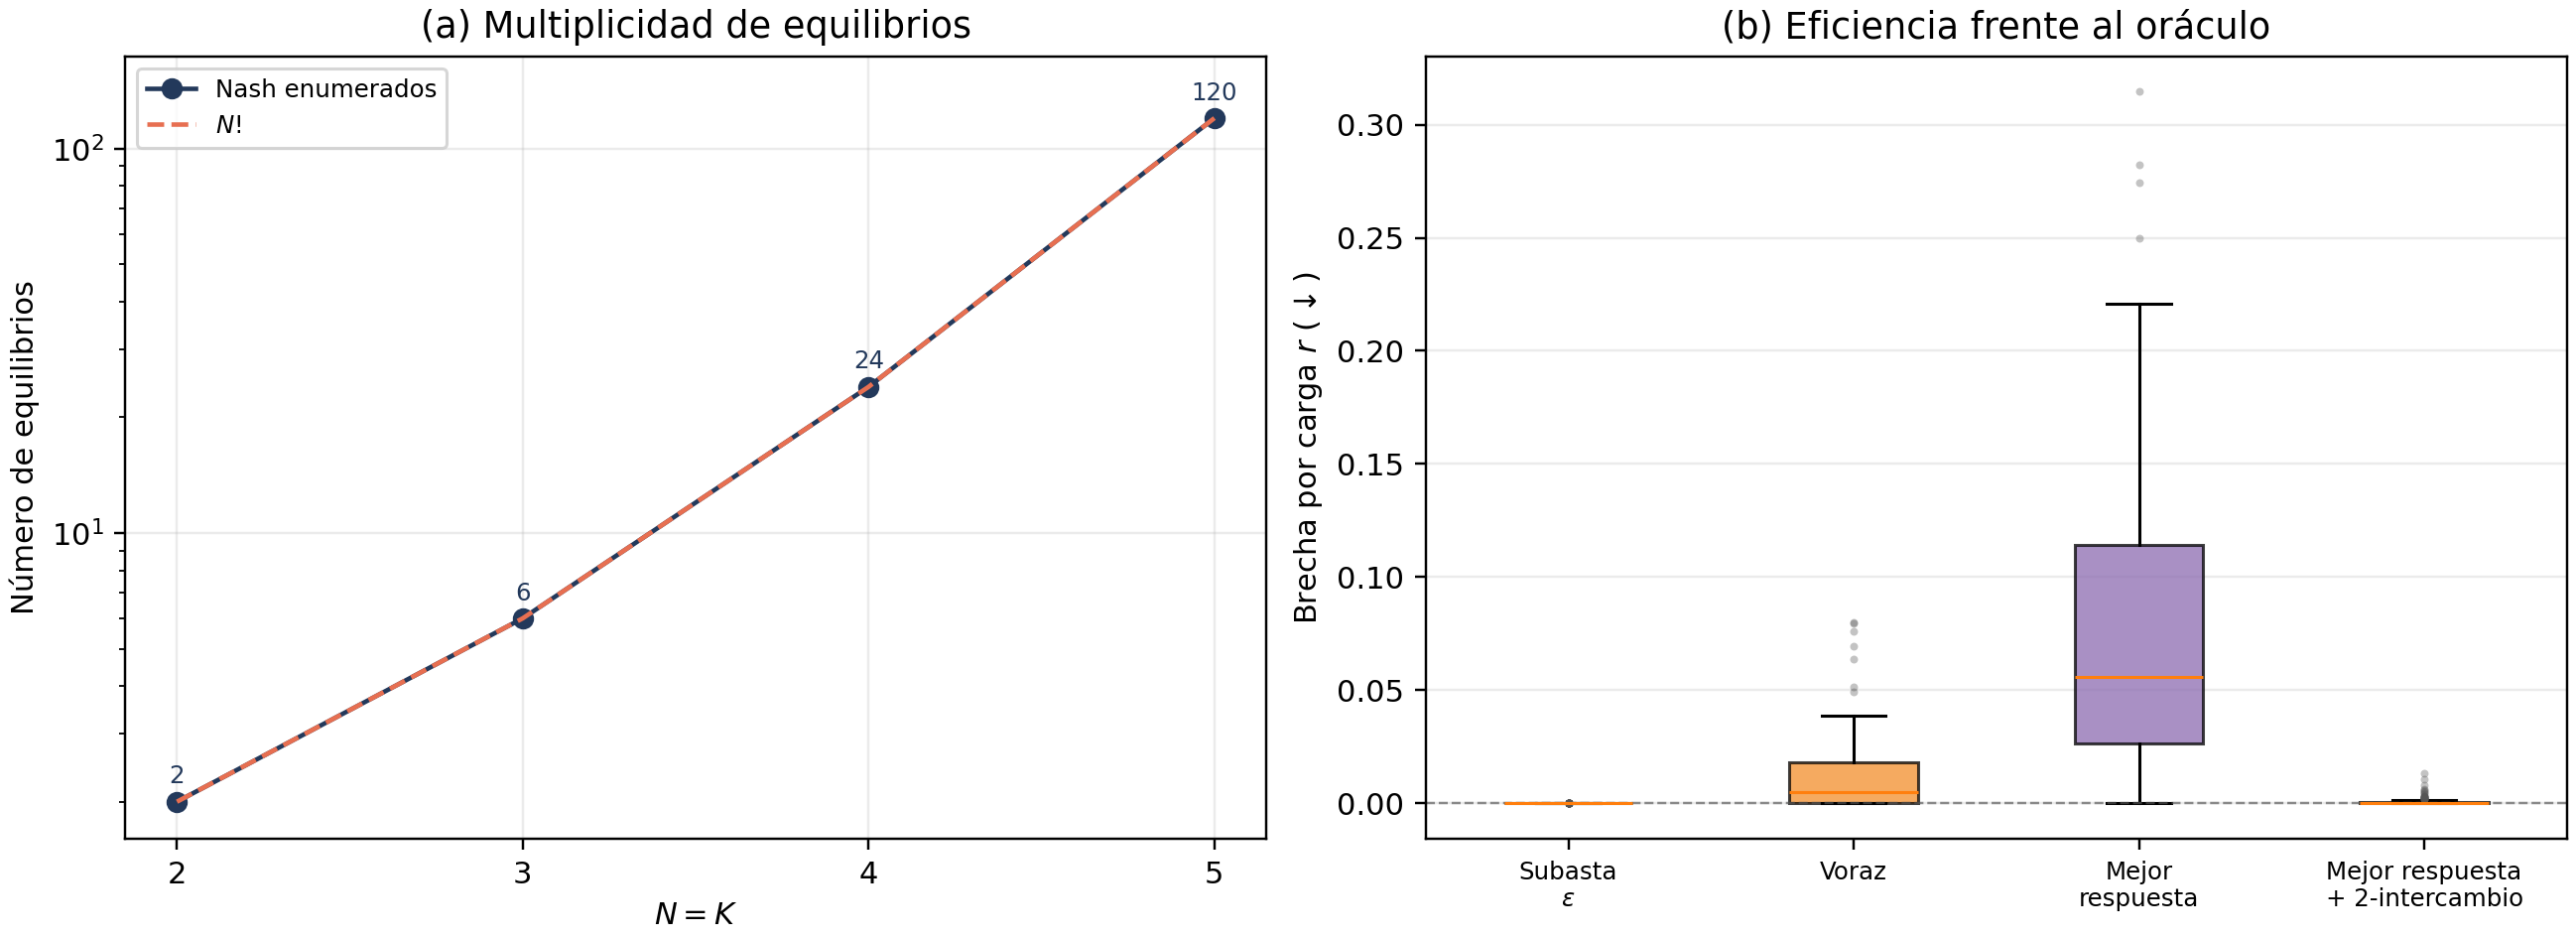
\includegraphics[width=0.96\textwidth]{../results/sp0/SP0_THEORY_v1/figures/fig-sp0-equilibrium-efficiency.pdf}
 \caption{SP0: (a) Nash enumerados frente a $N!$ en casos cuadrados. (b) distribución de la brecha por carga respecto al algoritmo húngaro en 200 instancias pareadas. Las cajas muestran el rango intercuartílico, la línea la mediana, los bigotes $1.5$ veces dicho rango y los puntos los valores atípicos.}
 \label{fig:sp0-equilibrium-efficiency}
 \viuownsource
\end{figure}
\fi

\paragraph{Factibilidad y eficiencia.}
El algoritmo húngaro, la subasta-$\varepsilon$, el método voraz, la mejor respuesta y la mejor respuesta con 2-intercambio fueron factibles en las 200 instancias, resultado coherente con la estructura del problema y, para mejor respuesta, con la proposición. La Tabla~\ref{tab:sp0-results} cuantifica la selección dentro del conjunto factible.

\begin{table}[!htbp]
 \centering
 \caption{Resumen agregado de los cinco métodos. La última columna contiene operaciones específicas de cada algoritmo y no una unidad común de complejidad.}
 \label{tab:sp0-results}
 \scriptsize
 \setlength{\tabcolsep}{3.7pt}
 \renewcommand{\arraystretch}{1.08}
 \begin{tabular}{lrrrr}
\toprule
Método & Factible [\%] & Brecha/carga mediana & $100W/W^\star$ & Op. registradas \\
\midrule
Hungarian (oráculo) & 100.0 & 0.0000 & 100.00 & 192 \\
Subasta $\varepsilon$ & 100.0 & 0.0000 & 100.00 & 9328 \\
Greedy & 100.0 & 0.0052 & 99.38 & 192 \\
Mejor respuesta & 100.0 & 0.0560 & 93.65 & 416 \\
Mejor respuesta + 2-intercambio & 100.0 & 0.0000 & 100.00 & 1116 \\
\bottomrule
\end{tabular}

 \viuownsource
\end{table}

Los valores no forman una clasificación arquitectónica porque los métodos reciben información distinta. Bajo ocupación coherente, mejor respuesta alcanzó siempre factibilidad, pero presentó una brecha mediana de $0.0560$ por carga y bienestar mediano del $93.65\%$. La diferencia pareada $r_{\mathrm{2-int}}-r_{\mathrm{BR}}$ fue $-0.07318$ (IC del $95\%$: $[-0.08201,-0.06508]$). El intercambio redujo la pérdida y obtuvo mediana cero, pero su cuartil superior fue $0.00065$. Este resultado no permite declarar optimalidad global. La subasta-$\varepsilon$ quedó prácticamente superpuesta al oráculo: diferencia media $5.74\times10^{-6}$ por carga (IC del $95\%$: $[3.37, 8.64]\times10^{-6}$), dentro de la cota aditiva.

\paragraph{Ablación de la penalización.}
La formulación con $\lambda>\kappa_{\max}$ produjo 200 asignaciones factibles de 200, mientras $\lambda=0$ no produjo ninguna. Las 200 discordancias favorecieron al mecanismo completo y McNemar exacto rechazó la igualdad de factibilidad ($p=1.24\times10^{-60}$). Sin recompensa de cobertura ni penalización de duplicidad, la inactividad domina frente a asociaciones de coste positivo. La ablación verifica la respuesta a los términos de déficit y exceso, pero no demuestra cardinalidad variable ni comunicación vecinal. Los tiempos observados hasta $N=64$ tampoco demuestran escalabilidad asintótica.

\subsubsection{Síntesis}

El algoritmo húngaro resuelve exactamente el caso uno-a-uno y la subasta-$\varepsilon$ aproxima su coste. El juego potencial añade una propiedad distinta: con $\lambda>\kappa_{\max}$, sus equilibrios puros son precisamente las asignaciones factibles. La selección sigue abierta, pues la mejor respuesta puede terminar en un equilibrio subóptimo. El 2-intercambio reduce esa brecha sin garantizar optimalidad global. SP1 retira la demanda unitaria y SP2 la equivalencia de capacidades.
